\section{Introduction}\label{sec:intro}

The goal of the OpenDreamKit project \cite{ODKproposal:on} is to develop a generic Toolkit
that will enable Mathematicians (and scientists in general) to build so-called Virtual
Research Environments (VREs) that are optimally tailored to specific communities. These
will combine a multitude of different tasks, such as symbolic mathematics, automatic code
generation, numerical computation, data bases, post-processing or visualisation. A VRE
will provide end-users with a single tool-chain that can be used for most, if not all, of
their research.

To be able to build such a toolkit, we will need to combine three different aspects --
Data (D), Knowledge (K) and Software (S). Ultimately we want to create and make use of them
using a VRE; we want to model the real world, translate it into a set of mathematical
objects and computationally simulate and thereby explore them.

The \emph{Data Aspect} is commonly implemented in special databases as tables or lists of
numerical of symbolic data. The \emph{Systems Aspect} is reprented by mathematical
software systems, such as \GAP, \SageMath, and others computing on top of this data. The
\emph{Knowledge Aspect} specifies the meaning of the mathematics data as well as the
knowledge underlying the algorithms and thus bridges between the former two. An
illustration with more examples of these aspects can be found in
Figure~\ref{fig:thebigpicture}.

\begin{figure}[H]\centering
  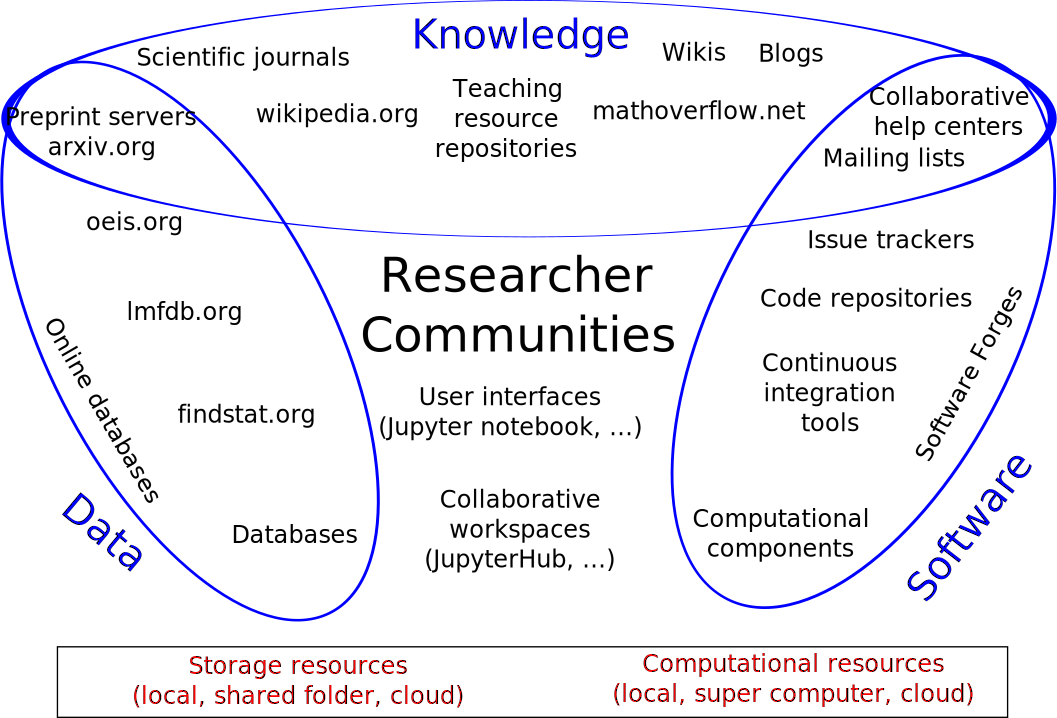
\includegraphics[width=\textwidth]{../../Proposal/Pictures/TheBigPicture.pdf}
  \caption{Virtual Research Environments for research in pure
    mathematics and applications.}
  \label{fig:thebigpicture}
\end{figure}

To achieve the task of building a VRE with these three aspects we want to use the
well-established framework of theory graphs -- which we will briefly explain below in
\ref{sec:MMT}. As a basis towards building DKS theories we use the \MMT system -- our
existing implementation of theory graphs -- which has K(nowledge) theories already. We
split the remaining task in two, integrating \textit{systems and knowledge}
(Section~\ref{sec:mitm}) and integrating \textit{knowledge and data}
(Section~\ref{sec:introfinal}).

\subsection{A Brief Recap of Theory Graphs}\label{sec:MMT}

A theory graph consists of theories and the relations between them. A theory in this sense
is a set of declarations -- a set of declared symbols. In addition to the declarations,
each theory has a name (which together with its namespace forms the global URI for the
theory) and a meta-theory. A meta-theory is commonly the logical framework that is used to
model the content of the theory. Each declared symbol has a name and can additionally have
a type, a definition and different kinds of meta-data. In each theory these symbols can
then be used to form terms that can be used to express more advanced knowledge. Here terms
are effectively OpenMath 2.0 \cite{BusCapCar:2oms04} objects -- they mostly consist of
literal values, symbols and applications of terms to other terms.

There are two basic kinds of relations between theories: imports and views. An import is a
way to declare symbols from one theory in another theory -- to import the symbols from a
source theory to a target theory. This can for example be used to extend an existing
theory without re-declaring all symbols or to combine two theories. Furthermore the
concept of imports allows to modularise knowledge. On top of imports there are also
Structures which are imports and additional renamings of the imported symbols. The second
type of relation, the view, is a mapping from one theory to another -- a way to ``view''
one theory as another. This mapping allows terms from one theory to be translated into
another theory. In the case where terms represent boolean statements or proofs, the
mapping given by the view is truth preserving -- \emph{i.e.}~if a statement is true in the
source theory, it is be true in the target theory after translation.

Theory graphs are implemented inside the \MMT system \cite{RabKoh:WSMSML13}. The system
allows for the declaration of theories along with symbols, imports and views. Furthermore
it is possible to create terms over these theories and translate them along views. The
\MMT system also provides a type checker that can be used to type check declarations.

\subsection{Using the Math-In-The-Middle approach to integrate systems}\label{sec:mitm}

When integrating multiple system we are mostly talking about using concrete algorithms
(implemented by these systems) to solve a specific computational problem (the knowledge
about the problem). To integrate multiple systems with this knowledge we want to enable
users to write down a problem in one system and then solve it in another system. We want
to be independent of the implementation of the knowledge -- independent of the systems.

For this we make use of an approach we call Math-In-The-Middle. Here the underlying
mathematical knowledge, the ``real math'', is in between (in the ``middle'') of the
systems -- hence the name. Each system needs access to this knowledge. As each of them
come with their own particularities, they will need some interface to it.

We want to make use of the modular approach to mathematics provided by theory graphs, and
in particular \MMT as an implementation thereof, to first of all allow us translate
mathematical expressions between systems. We define a ``Math In The Middle'' theory as
well as interface theories for each system. With the help of \MMT and bi-views\footnote{A
  bi-view is a bidirectional view between two theories} between the interface theories and
the central theory, we can translate objects from one system to the other.

\begin{figure}[ht]\centering
  \def\myxscale{3}\def\myyscale{1.2}
  \documentclass{standalone}
\usepackage[mh]{mikoslides}
% this file defines root path local repository
\defpath{MathHub}{/Users/kohlhase/localmh/MathHub}
\mhcurrentrepos{MiKoMH/talks}
\libinput{WApersons}
% we also set the base URI for the LaTeXML transformation
\baseURI[\MathHub{}]{https://mathhub.info/MiKoMH/talks}

\usetikzlibrary{backgrounds,shapes,fit,shadows,mmt}
\begin{document}
\begin{tikzpicture}[xscale=2.6,yscale=.9]
  \tikzstyle{withshadow}=[draw,drop shadow={opacity=.5},fill=white]
   \tikzstyle{database} = [cylinder,cylinder uses custom fill,
      cylinder body fill=yellow!50,cylinder end fill=yellow!50,
      shape border rotate=90,
      aspect=0.25,draw]
   \tikzstyle{human} = [red,dashed,thick]
   \tikzstyle{machine} = [green,dashed,thick]

\node[thy]  (mf) at (.2,5.3) {MathF};
\node[thy,dashed]  (compf) at (0,6) {CompF};
\node[thy,dashed]  (pf) at (-.9,5.5) {PyF};
\node[thy,dashed]  (cf) at (1,5.5) {C\textsuperscript{++}F};
\node[thy,dashed]  (sf) at (-0.9,4.6) {SAGE};
\node[thy,dashed]  (gf) at (1,4.6) {GAP};

\draw[include] (compf) -- (pf);
\draw[includeleft] (compf) -- (cf);
\draw[include] (pf) -- (sf);
\draw[includeleft] (cf) -- (gf);

\node[thy] (kec) at (0,3) {EC};
\node[thy,minimum height=.4cm] (kl) at (0,4) {\ldots};

\node[thy] (sec) at (-1,2) {SEC};
\node[thy,minimum height=.4cm] (sl) at (-1,3) {\ldots};

\node[thy] (gec) at (1,2) {GEC};
\node[thy,minimum height=.4cm] (gl) at (1,3) {\ldots};

\node[thy] (lec) at (-.3,1.2) {LEC};
\node[thy,minimum height=.4cm] (ll) at (.3,1.2) {\ldots};

\node (sc) at (-2,4) {SAGE};
\node[draw] (salg) at (-2,3.35) {Algo};
\node[database,dashed] (sdb) at (-2,2.4) {DB?};
\node[draw] (skr) at (-2,1.7) {KR};
\node[draw,machine] (sac) at (-2,1) {AbsClass};

\node (gc) at (2,4) {GAP};
\node[draw] (galg) at (2,3.35) {Algo};
\node[database,dashed] (gdb) at (2,2.4) {DB?};
\node[draw] (gkr) at (2,1.7) {KR};
\node[draw,machine] (gac) at (2,1) {AbsClass};

\node (lmfdb) at (0,0) {LMFDB};
\node[database] (ldb) at (1,-.4) {Mongo};
\node[draw] (knowls) at (-1,-.4) {Knowls};
\node[draw,machine] (lac) at (0,-.5) {AbsClass};

  \begin{pgfonlayer}{background}
    \node[draw,cloud,fit=(sec) (sl),aspect=.4,inner sep=-3pt,withshadow,purple!30] (st) {};
    \node[draw,cloud,fit=(gec) (gl),aspect=.4,inner sep=-4pt,withshadow,purple!30] (gt) {};
    \node[draw,cloud,fit=(kec) (kl),aspect=.4,inner sep=0pt,withshadow,blue!30] (kt) {};
    \node[draw,cloud,fit=(lec) (ll),aspect=2.5,inner sep=-7pt,withshadow,purple!30] (lt) {};
  \end{pgfonlayer}

\begin{pgfonlayer}{background}
  \node[draw,withshadow,fit=(sc) (skr) (sac) (sdb),inner sep=1pt] {};
  \node[draw,withshadow,fit=(gc) (gkr) (gac) (gdb),inner sep=1pt] {};
  \node[draw,withshadow,fit=(lmfdb) (lac) (ldb) (knowls),inner sep=1pt] {};
\end{pgfonlayer}

\draw[view] (kec) -- (sec);
\draw[view] (kec) -- (gec);
\draw[view] (kec) -- (lec);
\draw[include] (kec) -- (kl);
\draw[include] (gec) -- (gl);
\draw[include] (sec) -- (sl);
\draw[include] (lec) -- (ll);
\draw[view] (kl) -- (sl);
\draw[view] (kl) -- (gl);
\draw[view] (kl) to[bend left=5] (ll);

\draw[meta] (mf)  to [bend right=10] (st);
\draw[meta] (sf) -- (st);
\draw[meta] (mf)  to [bend left=10] (gt);
\draw[meta] (gf) -- (gt);
\draw[meta] (mf) -- (kt);
\draw[meta] (compf) to[bend right=15] (kt);

\draw[human,->] (skr) -- node[above]{\scriptsize induce} (st);
\draw[human,->] (gkr) -- node[above]{\scriptsize induce} (gt);
\draw[human,->] (knowls) -- node[left,near end]{\scriptsize induce} (lt);

\draw[machine,->] (gt) to[bend right=30] node[below,near start]{\scriptsize generate} (gac);
\draw[machine,->] (st) to[bend left=30] node[below,near start]{\scriptsize generate} (sac);
\draw[human,->] (st) to[bend left=20] node[below]{\scriptsize refactor} (kt);
\draw[human,->] (gt) to[bend right=20] node[below]{\scriptsize refactor} (kt);
\draw[human,->] (lt) -- node[right]{\scriptsize refactor} (kt);
\end{tikzpicture}
\end{document}
%%% Local Variables: 
%%% mode: latex
%%% TeX-master: t
%%% End: 

  \caption{The MitM paradigm in detail. PyF, C${}^{++}$F and CompF are (basic)
    foundational theories for \python, C${}^{++}$ and a generic computational model. SEC,
    LEC and GEC are theories for \SageMath, \LMFDB and \GAP elliptic curves.}\label{fig:mitm}
\end{figure}

A sketch of the theory graph based on the example of elliptic curves can be found in
Figure~\ref{sec:mitm}. We will not go into details here -- we have already discussed the
approach in \cite{DehKohKon:iop16}. Instead we focus on the second part of the problem,
integrating Data with Knowledge.

\subsection{Data-Knowledge Theories as a step towards DKS}\label{sec:introfinal}

The theories currently implemented inside \MMT are very good at formalising a variety of
knowledge, however are limited when it comes to representing a big amount of data. They
are are effectively K(nowledge)-Theories. To build the OpenDreamKit VREs however we need
to be able to utilise them for Data and different systems as well. As an initial design
step towards this we need to expand the theory graph model with a concept of
Data-Knowledge theories -- this is what we will focus on in this report.

In Section~\ref{casestudy}, we will first of all present the different systems that are
most relevant to the OpenDreamKit project. Next in Section~\ref{sec:data} we describe in
detail our concept of Data-Knowledge theories, and our implementation thereof in
Section~\ref{sec:impl}. Continuing in Section~\ref{sec:cases} by showing and explaining
which databases we have integrated into our efforts already. Next we show in
Section~\ref{sec:querying} how we plan to enable users to query and make further use of
DK-theories before finally concluding with a short summary and outlook in
Section~\ref{sec:conclusion}.

%%% Local Variables:
%%% mode: latex
%%% TeX-master: "report"
%%% End:
